\documentclass[justified]{tufte-handout}
\usepackage{../braph2_tut}
%\geometry{showframe} % display margins for debugging page layout

\title{Pipeline for Comparison between Groups of Subjects with Connectivity Data}

\begin{document}

\maketitle

\begin{abstract}
\noindent
For \emph{connectivity data}, we will upload a file containing the pipeline with the different steps to compare two groups of subjects. The connectivity values could correspond to white matter integrity values derived from DWI data or pre-calculated coactivations maps obtained from fMRI data. This Tutorial explains how to perform group comparisons with this kind of data.
\end{abstract}

\tableofcontents

\fig{figure*}
	{fig:01}
	{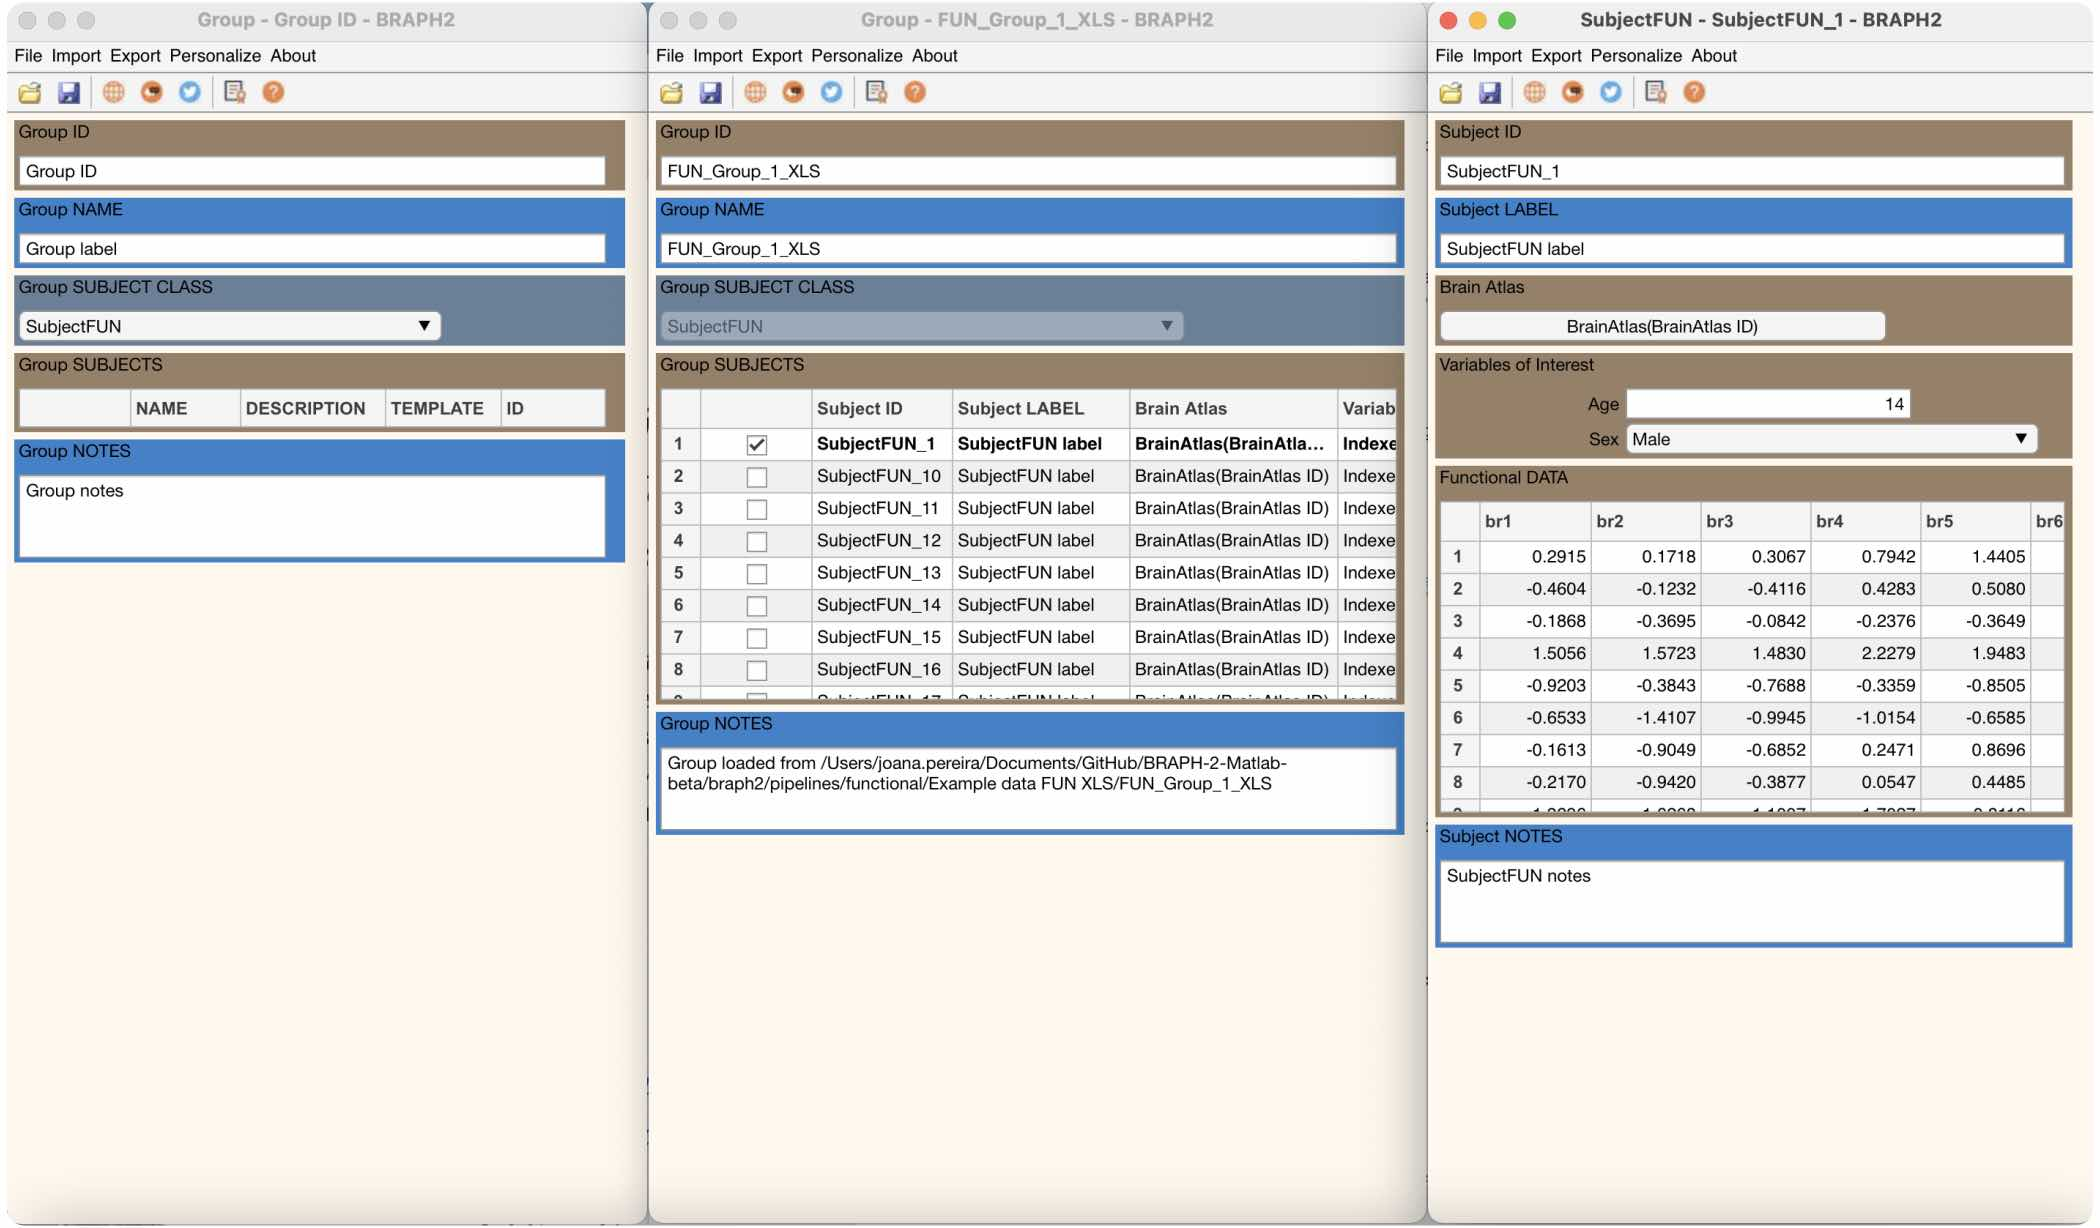
\includegraphics{fig01.jpg}}
	{GUI for working with the pipeline to compare two groups of subjects with connectivity files}
	{
	Full graphical user interface to perform group comparisons with connectivity data in BRAPH~2.0. 
	}

\clearpage
\section{Open the GUI}

The pipeline GUI can be opened by typing \code{braph2} in the MatLab's terminal, which allows you to select a pipeline (containing the steps required to perform your analysis), as shown in \Figref{fig:02}.

\fig{figure}
	{fig:02}
	{
	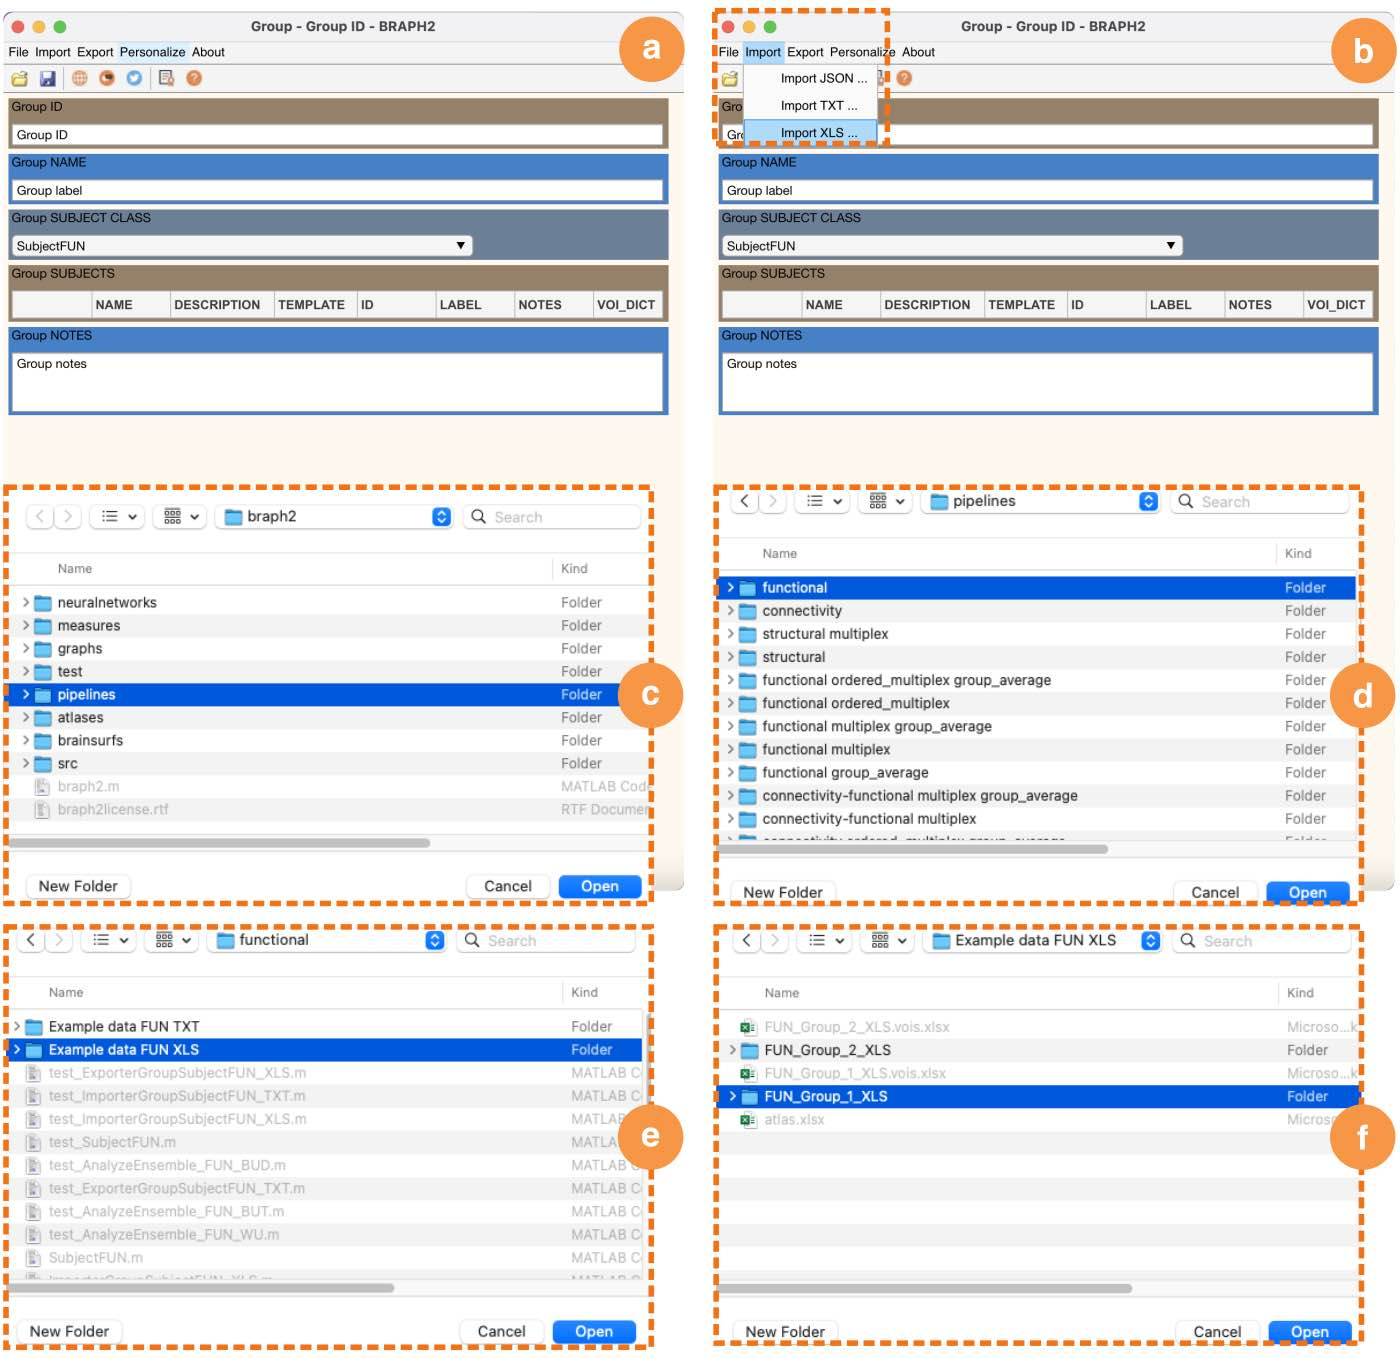
\includegraphics{fig02.jpg}
	}
	{Uploading the Connectivity Comparison Pipeline}
	{
	Steps to upload the pipeline to be able to compare two groups of subjects with connectivity data using the GUI: 
	{\bf a} Open the pipeline GUI.
	{\bf b} Import the file with the Weighted Undirected (WU) Connectivity Pipeline in JSON or BRAPH2 format.
	{\bf c}-{\bf e} Navigate to the BRAPH~2.0 folder \fn{pipelines}, {\bf d} \fn{connectivity}, and {\bf e} select the file  \fn{pipeline_connectivity_comparison_wu.braph2.
	}

To open the GUI and upload the connectivity comparison pipeline, you can also do it from the command line by typing the commands in \Coderef{cd:launch}.
%
\begin{lstlisting}[
	label=cd:launch,
	caption={
		{\bf Code to launch the GUI to upload a pipeline file to compare two groups of subjects.}
		This code can be used in the MatLab command line to launch the GUI to upload a pipeline file.
	}
]
pip = Pipeline(); ¥\circled{1}\circlednote{1}{creates a new object \code{Pipeline} to upload the steps to perform an analysis or comparison.}¥

gui = GUIElement('PE', pip); ¥\circled{2}\circlednote{2}{creates a GUI to upload the files into the pipeline.}¥
gui.get('DRAW')¥\circled{3}\circlednote{3}{draws the GUI.}¥
gui.get('SHOW') ¥\circled{4}\circlednote{4}{shows the GUI.}¥
\end{lstlisting}


Once the pipeline is uploaded, the GUI shown in (\Figref{fig:02}a) will contain different options to upload a brain atlas, upload the connectivity data of two groups, analyse them, and finally compare the groups (\Figref{fig:03}a). 

\section{Load the Brain Atlas}

\Figref{fig:03} shows how to upload the brain atlas that you used to extract the connectivity data for your analysis.

\fig{figure}
	{fig:03}
	{
	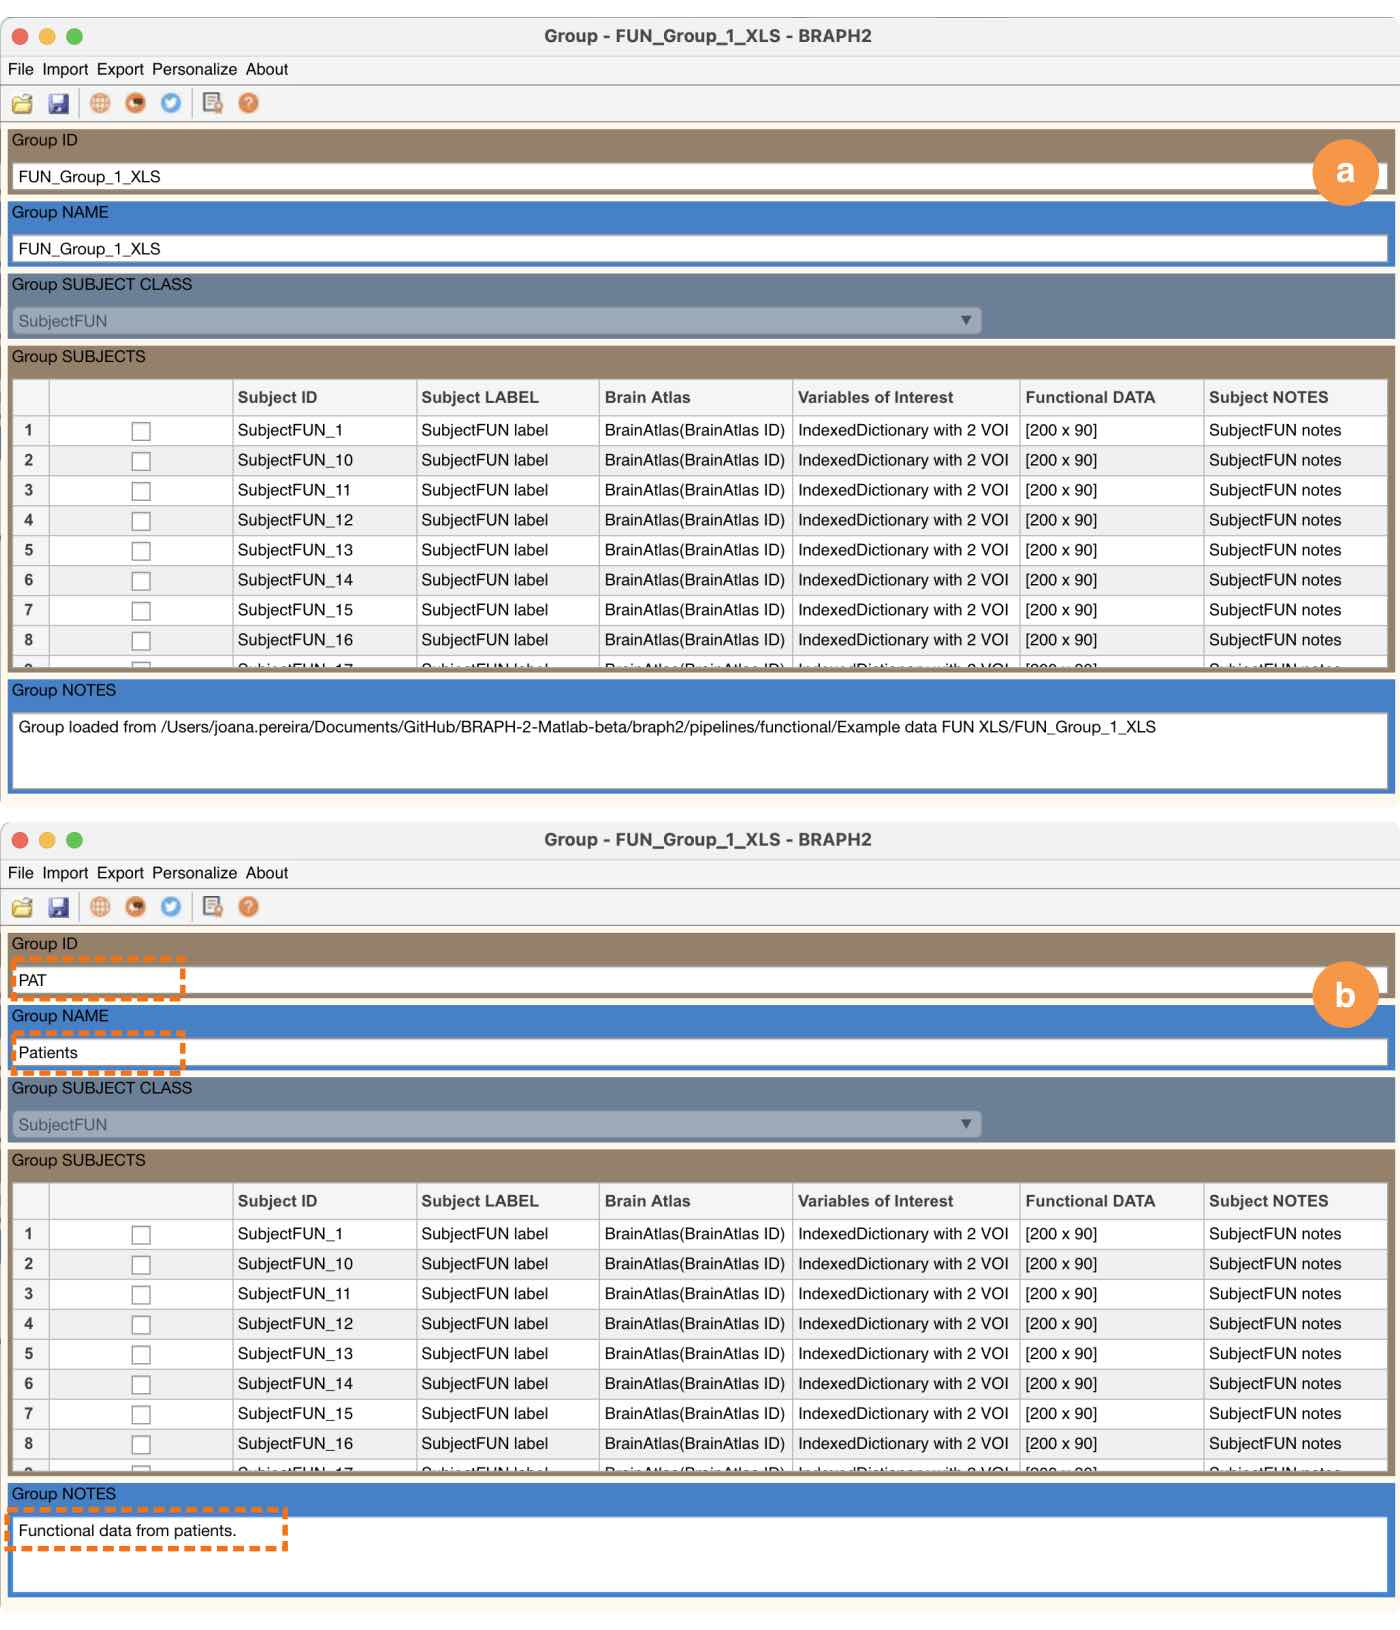
\includegraphics{fig03.jpg}
	}
	{Uploading the Brain Atlas}
	{
	Steps to upload the brain atlas:
	{\bf a} Click on \fn{Load Atlas} from the pipeline GUI.
	{\bf b} Navigate to the BRAPH~2.0 folder \fn{atlases} and {\bf c} select one of the atlas files, in this example the \fn{desikan_atlas.xlsx}. Similarly to the other tutorials, you can edit the information of this atlas as desired, including the Brain Atlas ID, NAME, NOTES or Brain Regions.

\section{Load the Connectivity Group Data}

After you loaded the brain atlas, you can upload the connectivity files for each group of subjects separately as shown in \Figref{fig:04}. A new window will be shown containing the data for the group you just selected. You can open each subject’s connectivity matrix by selecting
the subject, right click, and select “Open selection” (\Figref{fig:04}f), which shows the matrix values (\Figref{fig:04}g).	You should repeat the same procedure for group 2.
	
	\fig{figure}
	{fig:04}
	{
	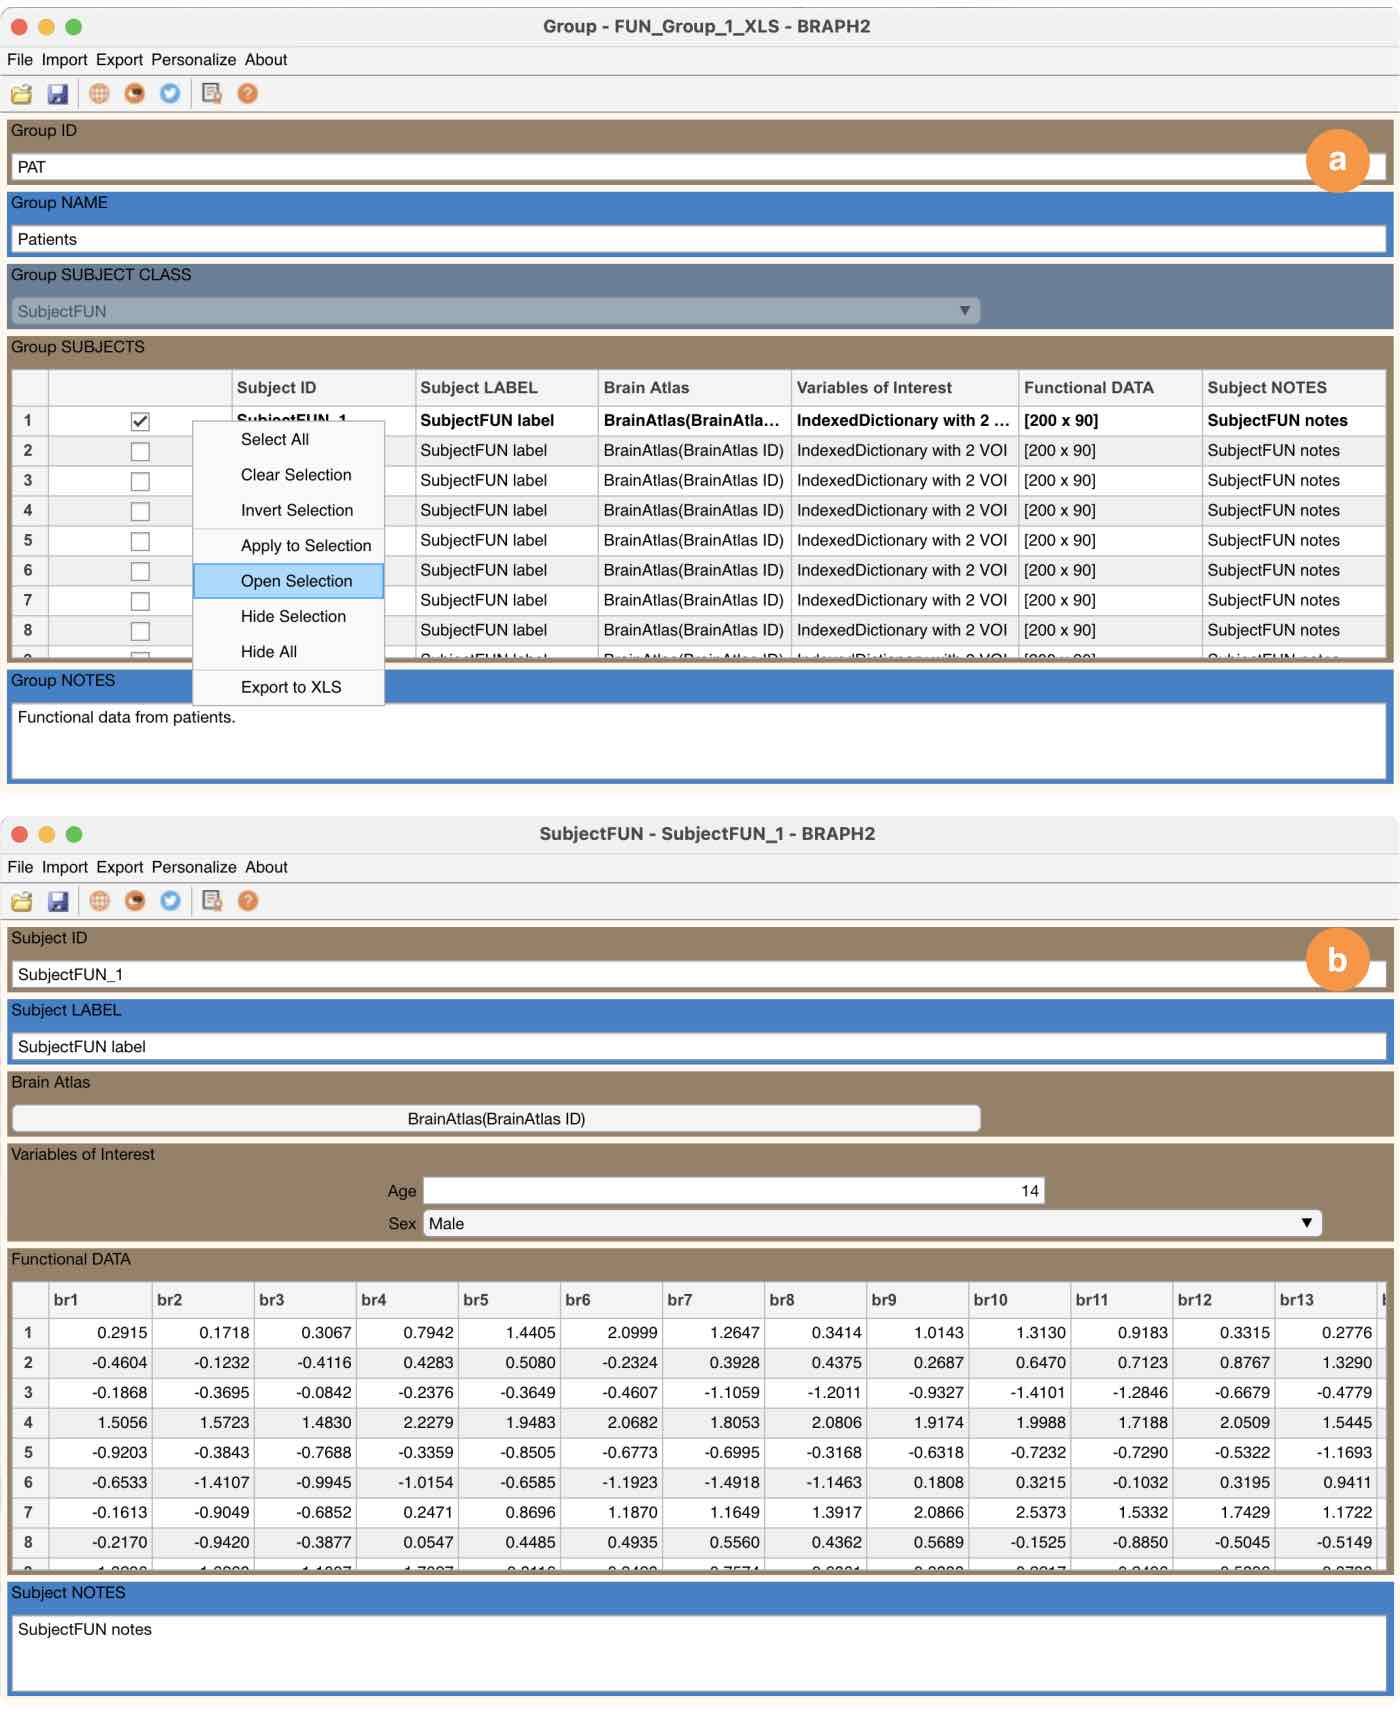
\includegraphics{fig04.jpg}
	}
	{Loading the Group Data}
	{
	Steps to upload the data from each group:
	{\bf a} Click on \fn{Load Group CON 1 from XLS from the pipeline GUI}.
	{\bf b} Navigate to the BRAPH~2.0 folder \fn{pipelines}, {\bf c} \fn{connectivity}, {\bf d} \fn{Example data CON XLS}, and select the folder {\bf e} \fn{CON\_Group\_1\_XLS}.

If you don't have the \fn{Example data CON XLS} folder inside \fn{connectivity}, then you can generate it by running the commands in \Coderef{cd:exampledata}.

\section{Analysing the Group Data}

Before running a group comparison, you must first click on \fn{Analyze Group 1} and \fn{Analyze Group 2} (\Figref{fig:05}a). Once you click on each of these options a new window will be shown that allows you to pre-calculate network measures for each group and explore them (\Figref{fig:05}b). This might be useful to get an insight on what these measures look like for each group.

	\fig{figure}
	{fig:05}
	{
	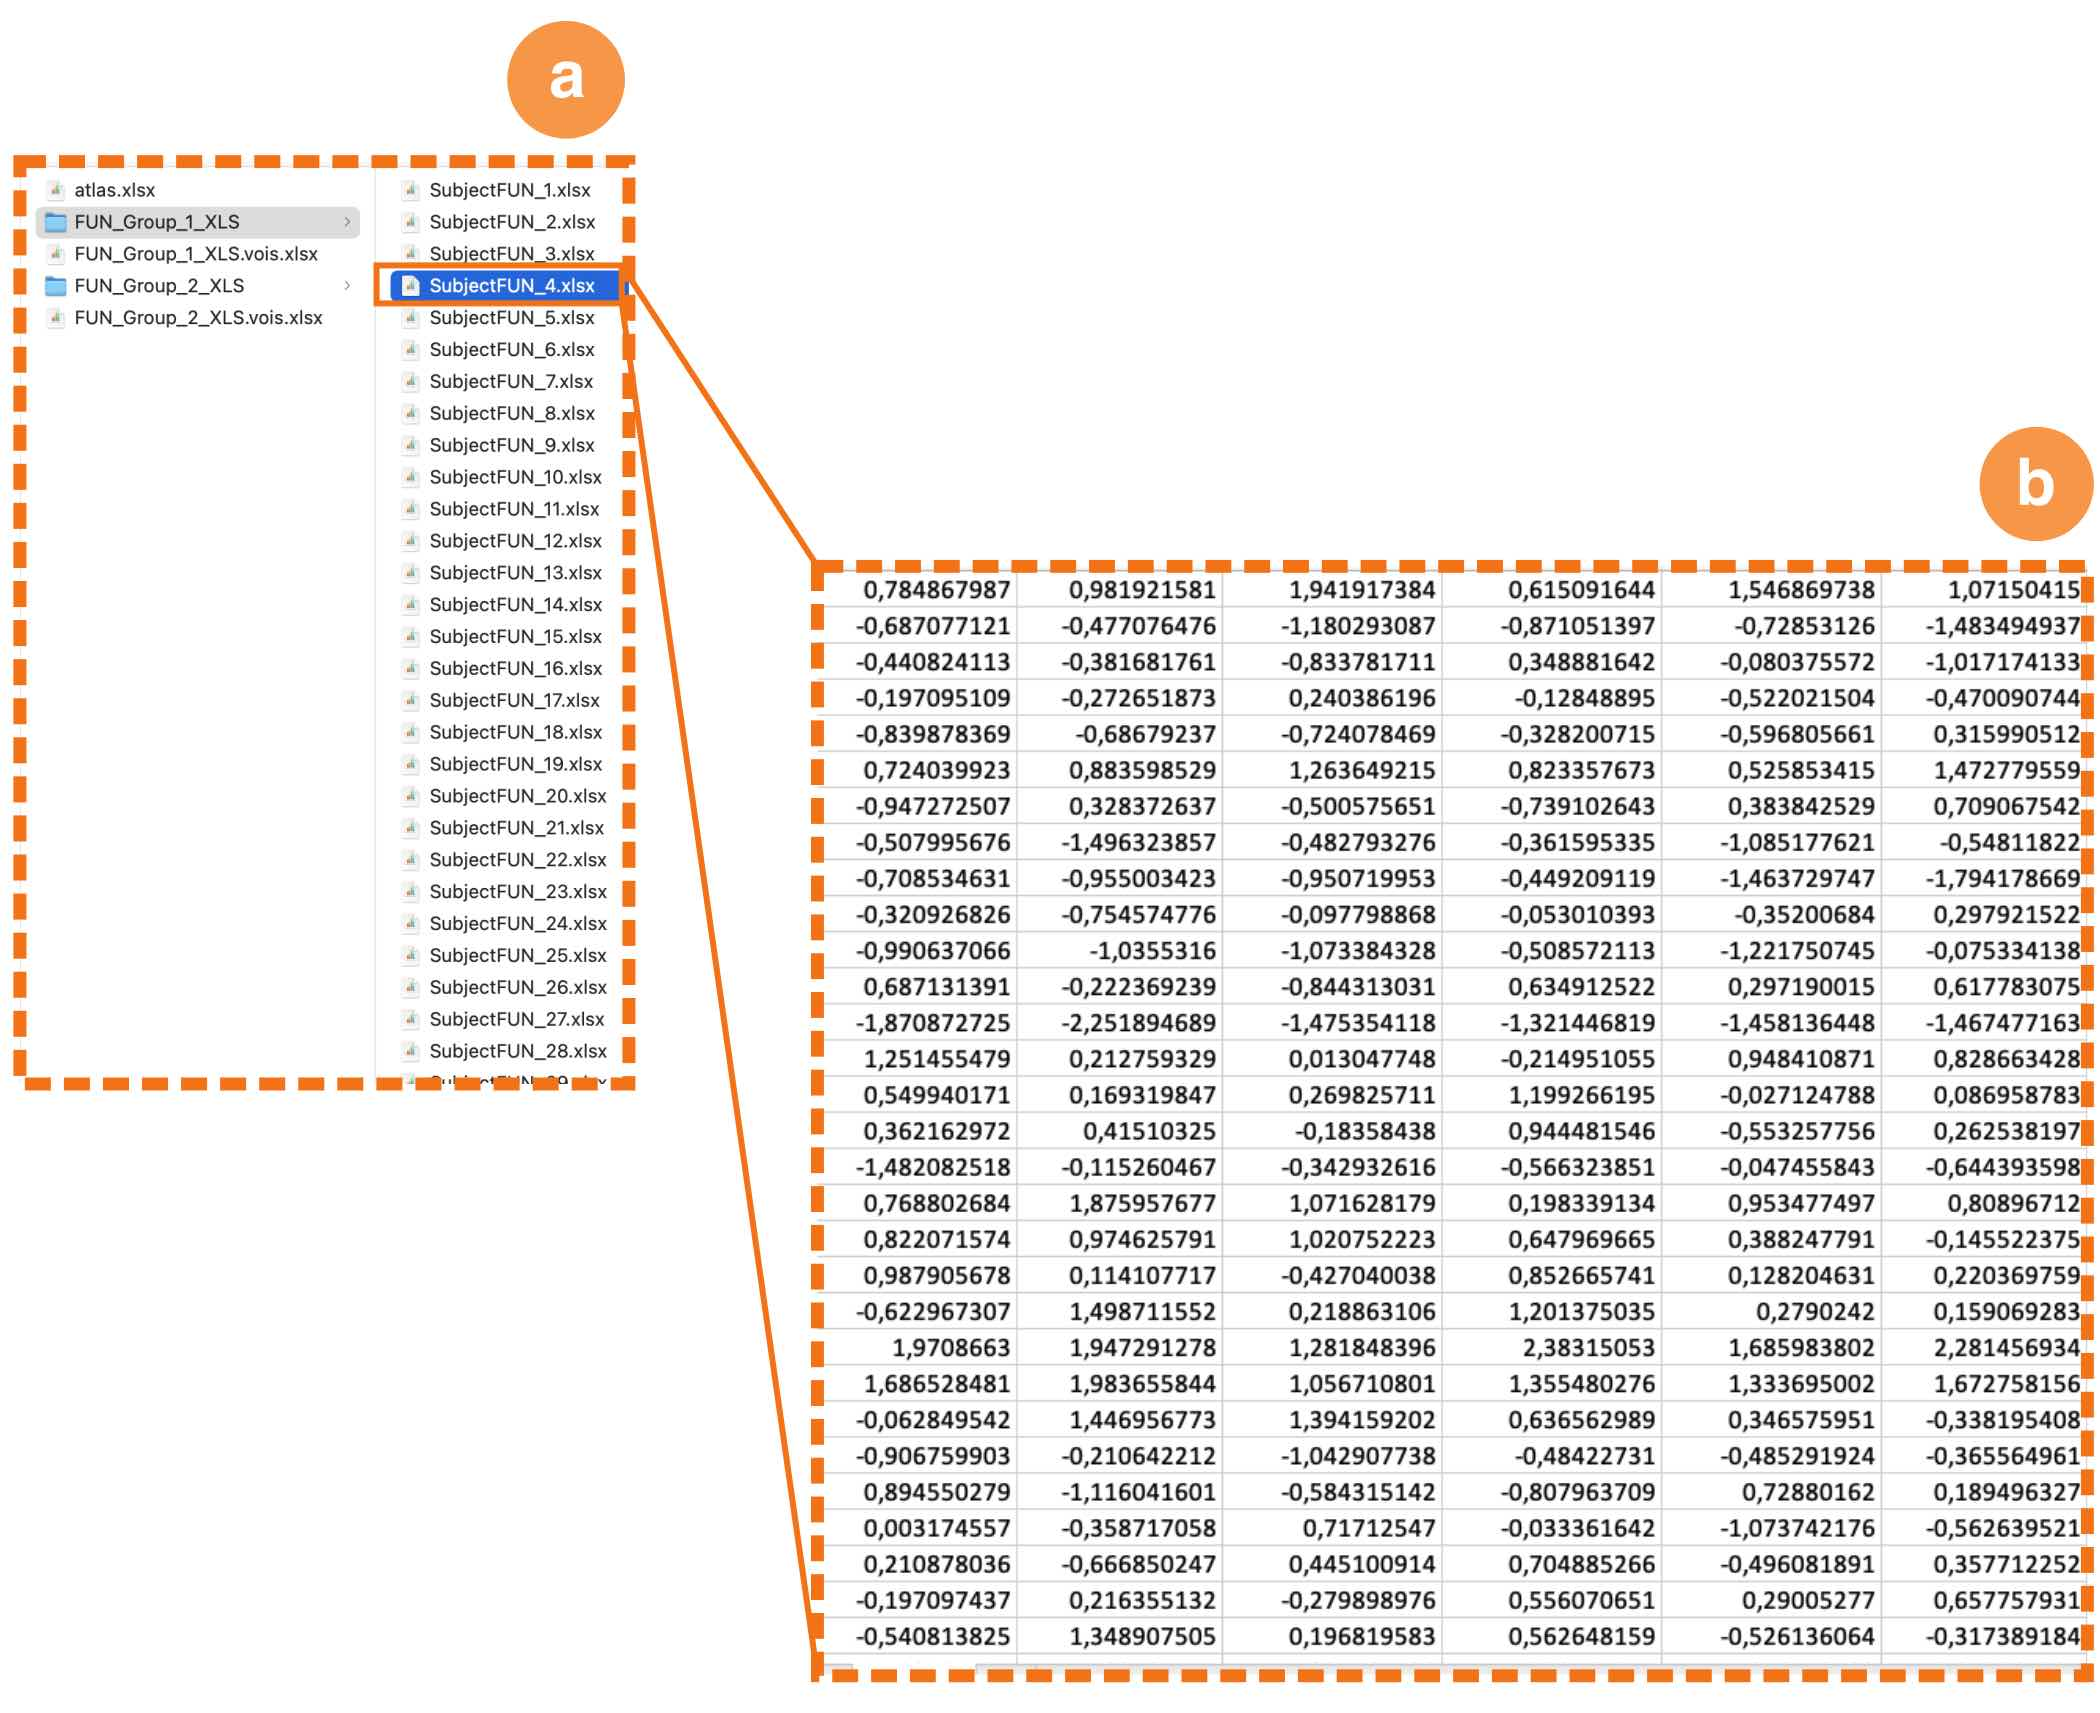
\includegraphics{fig05.jpg}
	}
	{Analyze the Group Data}
	{
	{\bf a} Click on \fn{Analyze Group 1} in the pipeline's GUI.
	{\bf b} In this new window, you can select different graph measures (... )

\section{Comparing Groups}

Once you have explored the network measures for each group, you can proceed with their statistical comparison. To do this, you should click on \fn{Compare Groups} (\Figref{fig:06}a) and in the window select (...) (\Figref{fig:06}b)

\end{itemize}	

\end{document}